%%%%%%%%%%%%%%%%%%%%%%% file template.tex %%%%%%%%%%%%%%%%%%%%%%%%%
%
% This is a template file for Web of Conferences Journal
%
% Copy it to a new file with a new name and use it as the basis
% for your article
%
%%%%%%%%%%%%%%%%%%%%%%%%%% EDP Science %%%%%%%%%%%%%%%%%%%%%%%%%%%%
%
%%%\documentclass[option]{webofc}
%%% "twocolumn" for typesetting an article in two columns format (default one column)
%
\documentclass{webofc}
\usepackage[varg]{txfonts}   % Web of Conferences font
%
% Put here some packages required or/and some personnal commands
%
%
\begin{document}
%
\title{Reaching new peaks for the future of the CMS HTCondor Global Pool}
%
% subtitle is optionnal
%
%%%\subtitle{Do you have a subtitle?\\ If so, write it here}

\author{
        \firstname{A.} \lastname{P\'erez-Calero Yzquierdo}\inst{1,2} \fnsep\thanks{\email{aperez@pic.es}} \and
        \firstname{M.} \lastname{Mascheroni}\inst{3} \and
        \firstname{M.} \lastname{Acosta Flechas}\inst{4} \and
        \firstname{J.} \lastname{Dost}\inst{3} \and
        \firstname{S.} \lastname{Haleem}\inst{5} \and
        \firstname{K.} \lastname{Hurtado Anampa}\inst{6} \and
        \firstname{F. A.} \lastname{Khan}\inst{4} \and
        \firstname{E.} \lastname{Kizinevi\v{c}}\inst{7} \and
        \firstname{N.} \lastname{Peregonov}\inst{4}, for the CMS Collaboration.
}

\institute{
    Centro de Investigaciones Energ\'eticas, Medioambientales y Tecnol\'ogicas (CIEMAT), Madrid, Spain \and
    Port d'Informaci\'o Cientifica (PIC), Barcelona, Spain \and
    University of California San Diego, La Jolla, CA, USA\and
    Fermi National Accelerator Laboratory, Batavia, IL, USA \and
    National Centre for Physics, Islamabad, Pakistan \and
    University of Notre Dame, Notre Dame, IN, USA \and
    European Organization for Nuclear Research, Meyrin, Switzerland
%    Vilnius University, Vilnius, Lithuania \and
}

\abstract{%
The CMS experiment at CERN employs a distributed computing infrastructure to satisfy its data processing and simulation needs. The CMS Submission Infrastructure team manages a dynamic HTCondor pool, aggregating mainly Grid clusters worldwide, but also HPC, Cloud and opportunistic resources. This CMS Global Pool, which currently involves over 70 computing sites worldwide and peaks at 350k CPU cores, is employed to successfully manage the simultaneous execution of up to 150k tasks. 
While the present infrastructure is sufficient to harness the current computing power scales, CMS latest estimates predict a noticeable expansion in the amount of CPU that will be required in order to cope with the massive data increase of the High-Luminosity LHC (HL-LHC) era, planned to start in 2027. 
This contribution presents the latest results of the CMS Submission Infrastructure team in exploring and expanding the scalability reach of our Global Pool, in order to preventively detect and overcome any barriers in relation to the HL-LHC goals, while maintaining high efficiency in our workload scheduling and resource utilization. 
}
%
\maketitle
% ---------------

\section{The CMS Submission Infrastructure}
\label{sec:intro}

The Submission Infrastructure (SI) team runs the computing infrastructure in which processing, reconstruction, simulation, and analysis of the CMS experiment physics data takes place. GlideinWMS~\cite{gwms} and HTCondor~\cite{htcondor} are employed in order to build a Global Pool~\cite{global_pool} of computing resources where these tasks are executed. The SI team also works on uncovering and solving operational limitations while preparing for future scales and requirements, the integration of new resource types and serving as liaison between the CMS collaboration and the HTCondor and GlideinWMS development teams, to stimulate cooperation and integrate new features as needed by the experiment.  

Achieving a successful scheduling of all CMS workloads requires taking in consideration their diversity and prioritization, along with their resource requirements. What constitutes successful scheduling is however subject to interpretation, namely ensuring that all available resources are efficiently used, a fair share of resources between groups of workload submitters, or the completion of tasks according to their prioritization, and with minimal job failures and manual intervention. The SI team is dedicated to ensuring that these potentially diverging goals are reasonably covered simultaneously.

The infrastructure employed by the SI team has evolved over the recent years towards a model of multiple interconnected HTCondor pools of resources (see Fig.\ref{complexity}). Specialized submission nodes ($schedds$), are deployed at CERN and FNAL. While being primarily attached to one of the pools, these schedds can however submit work into other federated pools, when resource demands are not covered by the primary one (a strategy known as $flocking$). For each pool, a Central Manager node is configured, running the $collector$ and $negotiator$ processes, services aggregating the latest status information of all slots in the pool and processing the matchmaking of job resource requests to open pool slots, respectively. 

The center piece of the model, the Global Pool, mainly acquires resources via the submission of GlideinWMS pilot jobs to WLCG sites~\cite{wlcg}. Pilot jobs, equivalent to resource requests on remote grid Compute Elements, are submitted by a number of distributed pilot $factories$ on behalf of the Front-End (FE) service, which processes the workload queue content to determine where resources should be acquired. The main pool can also include locally instantiated processing nodes ($startds$), for example via DODAS~\cite{dodas} or BOINC~\cite{boinc} (for the CMS@Home~\cite{lhcathome} project), and opportunistic resources such as the CMS High Level Trigger (HLT) farm~\cite{hlt} for offline processing when not in use for data taking. A number of CMS sites have also expanded their computing capacity by locally aggregating resources from High Performance Computing (HPC) facilities in a transparent way for CMS, as exemplified by the CNAF~\cite{cineca} and KIT~\cite{kit} cases, where pilot jobs arriving at the sites' compute elements are in turn rerouted to the HPC cluster batch system. This approach follows the CMS strategy to employ HPC resources whenever available~\cite{hpc}. A second HTCondor CERN pool includes the on-site CMS resources, as well as opportunistic BEER~\cite{beer} and Azure~\cite{azure} cloud slots. The HEPCloud~\cite{hepcloud} pool, joining cloud and HPC resources in the USA (e.g. at NERSC~\cite{nersc}), is managed from the FNAL site. Finally, additional external pools can be federated into the SI by enabling flocking from the CMS schedds.

\begin{figure}[ht]
\begin{center}
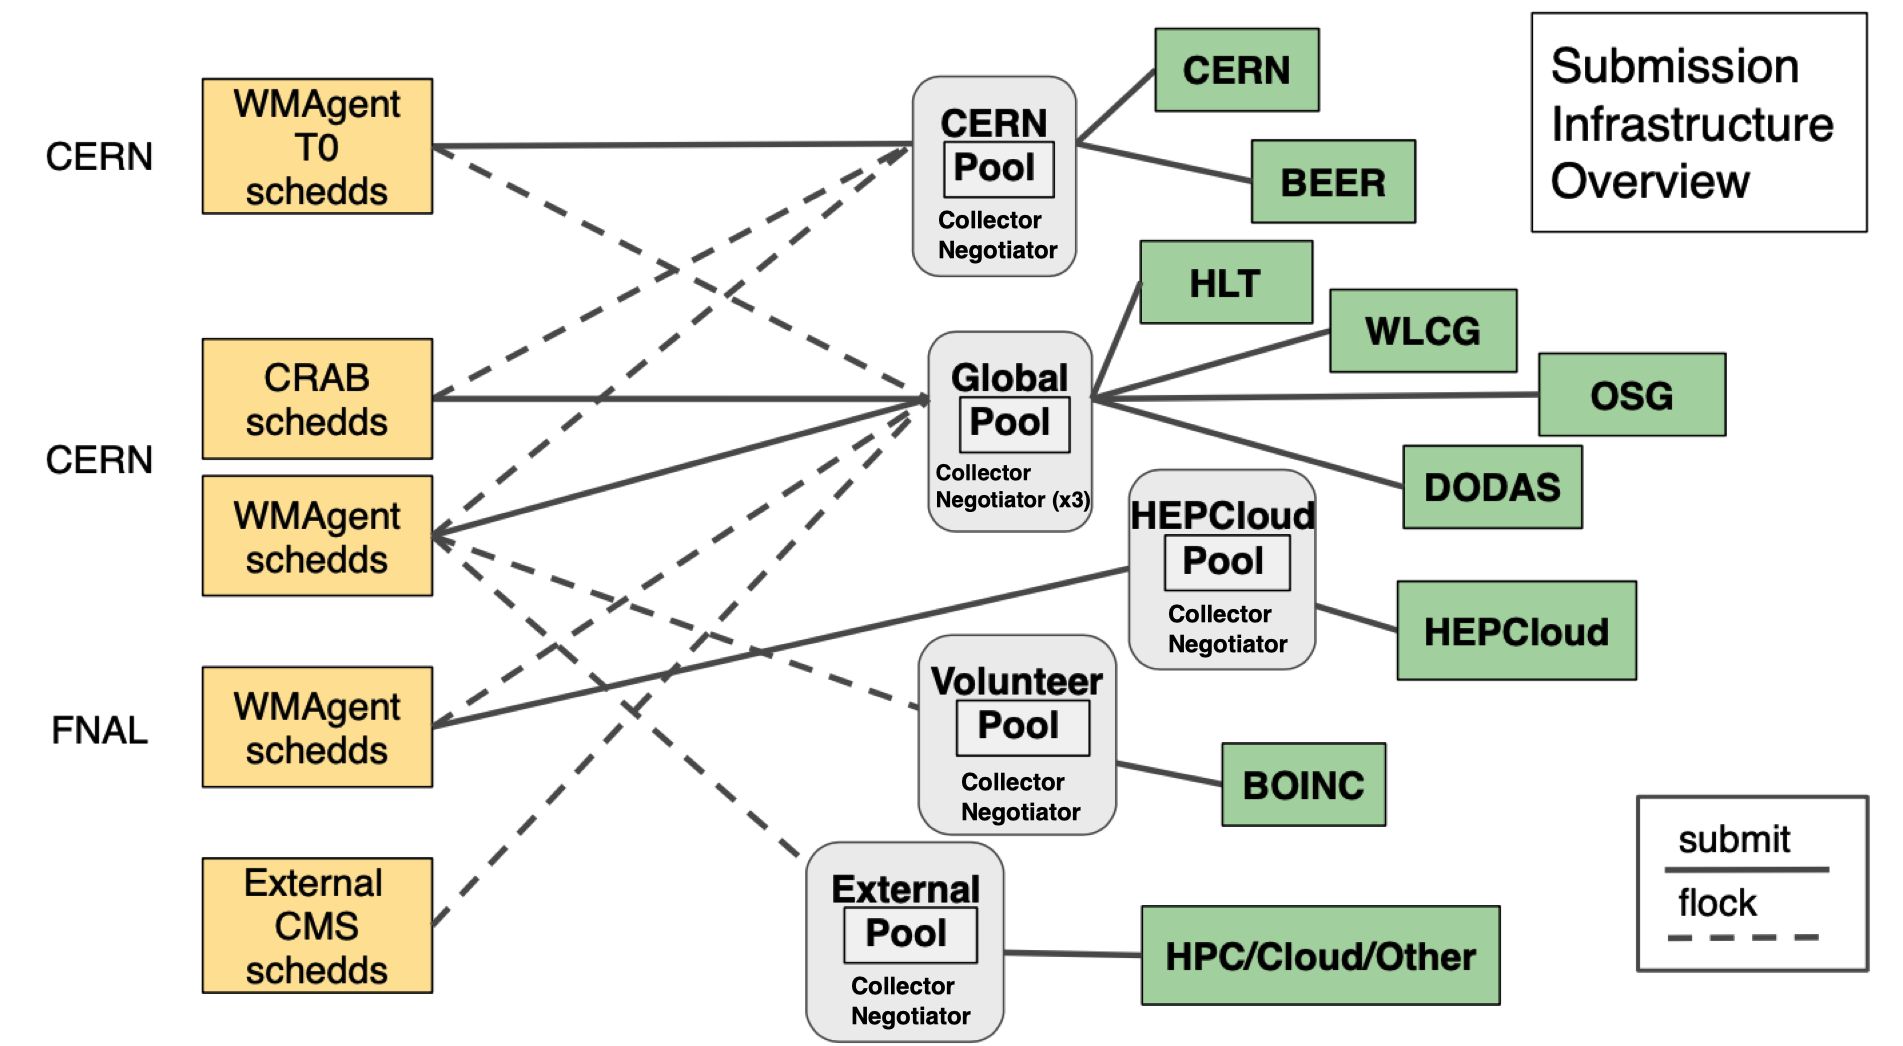
\includegraphics[width=10cm]{images/pool_complexity_2.png}
\setlength{\belowcaptionskip}{-20pt}
\caption{CMS SI current configuration, including multiple federated pools of resources allocated from diverse origins (green boxes) and sets of distributed job schedulers (schedds), handling the Tier 0 and centralized production workloads (WMAgent), as well as analysis job submission (CRAB).} 
\label{complexity}
\end{center}
\end{figure}

\section{Scalability requirements for the Global Pool}
\label{sec:reqs}
The Global Pool has been continuously growing in size over the last years, driven by the increasing resource requests during the LHC Run 2 (2015 to 2018), and through the Long- Shutdown 2 period (from 2019 to the present date), with the progressive incorporation of opportunistic and non-standard resources. Indeed, opportunistic, HPC and Cloud resources have been added to the Global Pool, currently aggregating over 300,000 CPU cores routinely, in an increasing proportion compared to the standard Grid sites slots, 

Considering the growing scales of data to be collected by CMS in the LHC High Luminosity (HL-LHC) phase, driven by increasing detector trigger rates and event complexity, CMS published in 2020 its estimated computational needs in the future~\cite{cms_hllhc} (see Fig.~\ref{cpu_needs}). As shown, a dramatic increase is anticipated for the second half of the 2020s compared to the current capacity and the moderate growth expected for the Run 3 years.

As presented also in Fig.~\ref{cpu_needs}, the CMS CPU demands will be at least a factor 4 or 5 higher than a simple extrapolation of the current capacity into the HL-LHC phase at fixed cost (i.e. from continuously evolving technologies at a rate of 10\% to 20\% yearly performance improvement). In addition to the expansion of the CMS infrastructure to new resource types and providers, the gap is also foreseen to be reduced by a number of R\&D projects currently being developed at the CMS software and data formats level~\cite{cms_RandD}. 

\begin{figure}[h]
\begin{center}
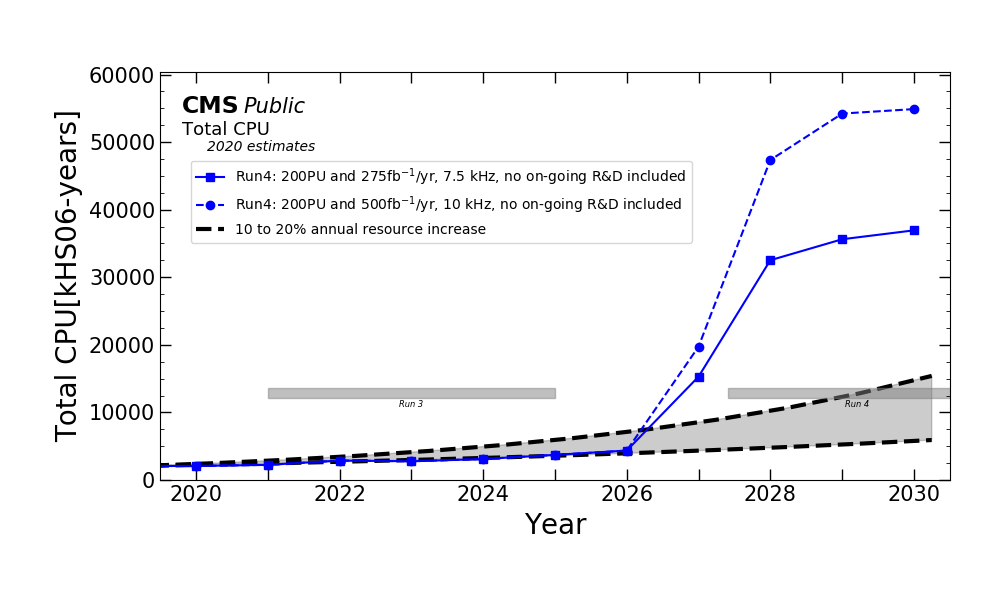
\includegraphics[width=10cm]{images/cpu_cms2020.png}
\setlength{\belowcaptionskip}{-20pt}
\caption{CMS CPU resource needs projections into the HL-LHC era, computed according to two scenarios of detector trigger rates and assuming a value of 200 for the pile-up (PU, the number or proton-proton collisions per LHC bunch crossing event).} 
\label{cpu_needs}
\end{center}
\end{figure}

Uncertainties about the future CMS CPU needs propagate into the SI domain, with basic matters such as the total amount of resources that SI will need to manage, how many simultaneous tasks would be executed or how many job schedulers will we have to employ in order to execute future workloads and make efficient use of such resources. Making predictions even harder, compute resources growth will unlikely come from increasing capacities at Grid sites, therefore further heterogeneity and specialization have to be considered as well. 

\section{Scalability tests}
\label{sec:test}
In order to preventively detect and solve potential scalability limitations, the SI group regularly conducts dedicated tests on the capacity for our infrastructure to grow while maintaining high efficiency and stability. Given the continuous evolution of our underlying tools, these tests have been executed recurrently over the last years (original tests described in~\cite{scale_2015}), involving a testbed HTCondor pool which is stressed to the limits of its capacity. As a canonical test, the number of simultaneously running tasks is progressively enlarged until the pool's performance degrades, for example in terms of reduced matchmaking efficiency or matchmaking processing time. These experiences are subsequently presented and discussed with the HTCondor and GlideinWMS development teams.

In previous test cycles, it was typically found that the collector of the pool was the limiting factor. Specifically, the collector capacity to process slot information updates saturates when the pool and the number of running tasks grow (determined by the collector daemon core duty cycle reaching 100\%). The collector performance limits have been again directly put to the test in the present scalability evaluation. Moreover, in addition to testing the capabilities of the latest HTCondor version available, we also want to compare test setups where the central manager of the pool is hosted on virtual versus physical machines. Finally, a test of the complete infrastructure was launched, which allows us to explore any limitations also on the GlideinWMS layer and in the available capacity of the scheduling nodes. These tests will be described in the following sections.

\subsection{Testing setup}
\label{sec:setup}
Our tests have explored the capacity and performance of a setup based on HTCondor 8.9.10, latest available version in the development series, while the test FE and factory services (requesting and submitting pilots) were running GlideinWMS 3.7.2.

In order to estimate the potential impact of the virtualization layer in degrading the performance of our collector, two hosts were employed: 
\begin{itemize}
    \item vocms0809: a virtual machine (VM), with 24 CPU cores, hosted on a node based on the Intel(R) Xeon(R) CPU E5-2650 v4 @ 2.20GHz processor, with 256 GB of RAM and 4 SSDs of 1.2 TB each. This node, in spite of being a VM, was not co-hosted with any other service at the time of the tests, so any performance reduction should come from the hypervisor technology (Openstack). 
    \item vocms0803: a physical machine (PM), with 32 cores, based on Intel(R) Xeon(R) Silver 4216 CPU @ 2.10GHz processor, with 187 GB of RAM and 2 SSDs of 1.8 TB each.
\end{itemize} 

Collector daemons were deployed on both nodes with an identical configuration. Finally, in order to provide job submission capacity to the test pool, a number of schedds (initially 10, later on 15) were installed on VMs running with 32 cores, 57 GB of RAM and 512 GB of High IO disk.

\subsection{Collector performance comparison with condor\_advertise}
\label{sec:advertise}

In the first stage of the tests, $condor\_advertise$ commands~\cite{advertise} were launched, which create a stream of slot update messages ($ads$) aimed at each of the two collectors. The total rate of slot updates submitted in parallel could be tuned by selecting the number of simultaneous advertising schedds, the number of parallel updates per schedd, the number of cycles and the sleep time between cycles. Communication was performed via UDP packets, which would accumulate at each node up to a total buffer size of 2 GB in both cases. Both collectors were tested, gradually increasing their stress, with slot update rates ranging from 60 to 180 ads/s. 

%first with the scale\_master.sh: 
%\begin{verbatim}
%#!/bin/bash
%
%#advertise sent in parallel
%NUM_SLAVES=20 
%
%date
%for ((i=0;i<$NUM_SLAVES;i++)); do
%   ./scale_slave.sh vocms0809 $i & # Load on the VM
%   ./scale_slave.sh vocms0830 $i & # Load on the PM
%done
%wait
%date
%\end{verbatim}

%Then, the code for the scale\_slave.sh algorithm employed was:
%\begin{verbatim}
%#!/bin/bash
%#Number of cycles, separated by a $SLEEP_TIME
%NUM_CYCLES=50000 
%
%COLLECTOR=$1
%SLAVE_ID=$2
%SLEEP_TIME=0.05
%#--- START SCALE TEST ---
%let cc=0 #cycle counter
%while [ "$cc" -lt $NUM_CYCLES ]; do
% sed "s/test0/test$RANDOM/" adv_file \
% |sed "s/test1/test$RANDOM/" |sed "s/test2/test$RANDOM/" \
% |sed "s/test3/test$RANDOM/" |sed "s/test4/test$RANDOM/" \
% |sed "s/test5/test$RANDOM/" |sed "s/test6/test$RANDOM/" \
% |sed "s/test7/test$RANDOM/" |sed "s/test8/test$RANDOM/" \
% |sed "s/test9/test$RANDOM/" | condor_advertise -multiple -debug \ 
% -pool $COLLECTOR.cern.ch:9618?sock=collector$((9621 + $RANDOM % 100))\
% UPDATE_MASTER_AD>/dev/null
%	sleep "$SLEEP_TIME"
%	let cc=cc+1
%done
%\end{verbatim}

The results of these tests, comparing the collector performance on the VM versus the PM, are summarized in Fig.~\ref{ad_tests}. A total of 4 stress test rounds were performed, corresponding to 60, 120, 180 and 90 ads/s respectively. The performance of the PM hosted collector is clearly superior, as saturation is only observed in the most extreme test, at 180 ads/s, in contrast to the VM hosted collector, reaching saturation in all cases, leading to UDP packets processing errors, which results in missed slot updates. At 120 ads/s, the PM collector is still viable, its duty cycle having reached around 75\%. UPD packet losses could only be measured in the case of 180 ads/s.  

\begin{figure}[h]
\begin{center}
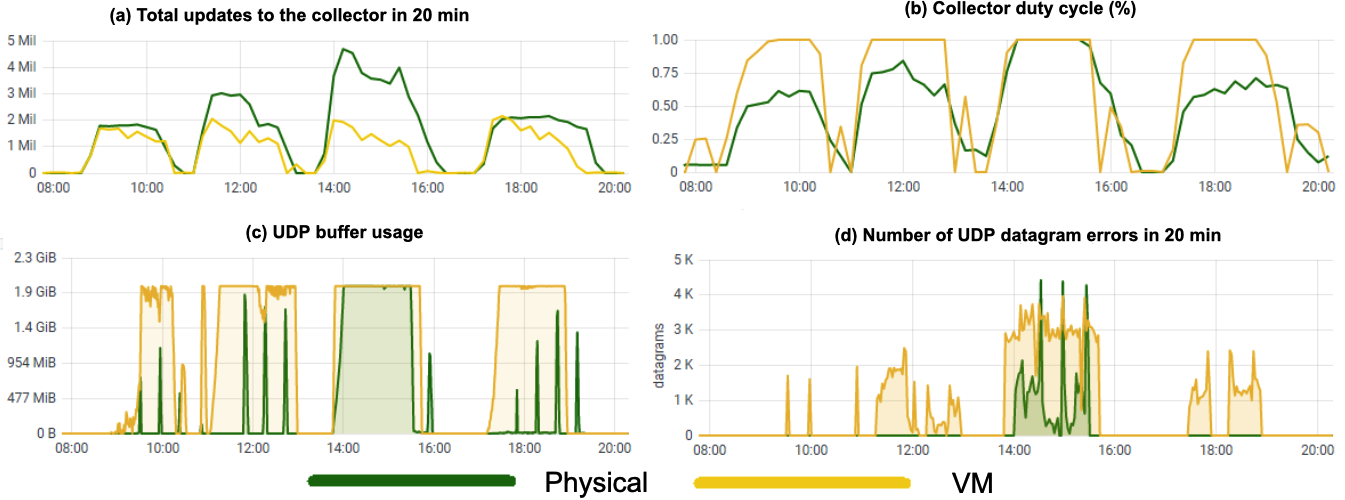
\includegraphics[width=13cm]{images/condor_advertise_tests_2.png}
\setlength{\belowcaptionskip}{-20pt}
\caption{Four rounds of condor\_advertise tests on the VM and PM collectors: (a) total number of updates processed over a 20 minutes integration window, (b) core duty cycle, (c) UDP buffer usage and (d) number of UPD packet errors in a 20 minutes integration window.} 
\label{ad_tests}
\end{center}
\end{figure}

\subsection{Full infrastructure test}
\label{sec:fulltest}
In order to explore increasingly larger scales, test pools can be simulated by running multiple multi-core startd daemons for each GlideinWMS pilot job running on the Grid ($uberglideins$, in contrast to one startd per glidein employed in the production pool~\cite{uberg}). This strategy has been successfully employed in previous iterations of our tests~\cite{scale_2015}.

Having analysed the results of the condor\_advertise tests, it was decided to explore the scalability limitation of the infrastructure focusing on the setup with the central manager of the test pool being hosted by the physical node, configured identically to the production Global Pool (e.g. running 3 negotiator instances in parallel). An initial set of 10 schedds (later on expanded to 15) were utilized to provide the job submission pressure on the pool. As in previous iterations, millions of jobs were injected in the schedd queues as single-core tasks. The stress on the collector is maximum when the pool is completely fragmented into single-core dynamically partititoned slots, hence the job parameter choice. Other job specifications, such as requested memory, disk, and site whitelist, are randomly generated within realistic values, to maximize job diversity and explore the matchmaking cycle length (negotiation time) on which the pool could efficiently operate. Job length is also selected with a realistic value of 8 hours with a gaussian dispersion of 2 hours. %, which can be tuned to force the job completion and submission rates in order to vary the degree of stress on the schedds. 

Several scale test rounds were launched, as Fig.~\ref{tests} shows. In the first phase, 10 schedds were employed, which was however determined to be insufficient in order to reach the target mark of 500,000 simultaneous running jobs. Indeed, memory usage of the submit nodes increases with the number of $shadow$ processes (one per running job to keep track of the its status on the remote execution slots), which in our setup limited the capacity of the schedds to manage running jobs to a maximum of 40k to 45k each. Thus, in the second phase, five more schedds were added to the pool for an increased job submission capacity. With the growth in running jobs and the subsequently enlarged pool, the maximum number of TCP sockets available in the condor connection broker (CCB) service was also reached. This caused that even if pilots were being submitted to grid sites, their slots could not be registered into the pool. Finally, in the third test round, having corrected all the previous limitations, and with 15 operative schedds, the 500,000 running jobs milestone was achieved, reaching a maximum of 590,000 jobs recorded at peak.

\begin{figure}[h]
\begin{center}
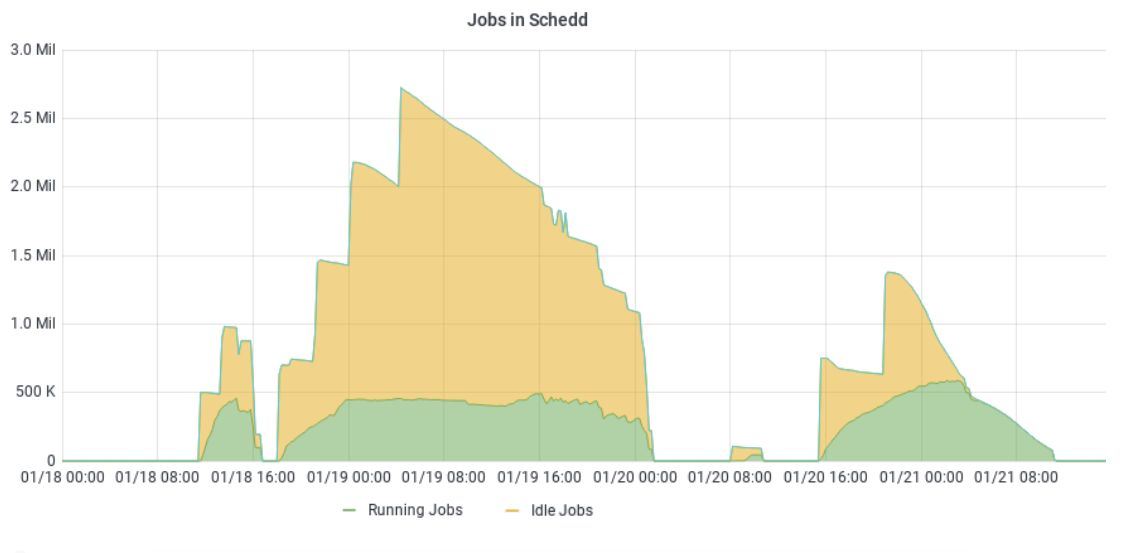
\includegraphics[width=12cm]{images/uberglidein_tests.png}
\setlength{\belowcaptionskip}{-20pt}
\caption{Number of simultaneously running and queued jobs for the scalability tests performed during January 2021 on the CMS HTCondor Global Pool. Successive attempts at reaching the 500,000 running jobs goal were performed under varying conditions, as described in the main text.} 
\label{tests}
\end{center}
\end{figure}

% ----------
\subsection{Overall evaluation of the test results}
\label{sec:results}
Having determined the clear advantage of the physical node over the VM as host to the collector and negotiator services, and with sufficient capacity to sustain a high enough jobs submission rate, the previously unattainable mark of 500,000 slots and jobs was surpassed. 

The plots in Fig.~\ref{collector} allows us to analyse the role of the collector as a limiting factor in the growth of the pool. We can observe how the collector core daemon duty cycle is correlated with both the total number of dynamic slots in the pool (each corresponding to one running task) and with the number of slot updates that need to be processed. The collector duty cycle saturates around 500,000 slots and with 1 million slot updates (integrated in a 20 minute window). 

Beyond that point, even though the collector remains active, its performance is severely degraded, which has a a number of consequences to the performance of the pool. One is immediately visible in Fig.~\ref{collector} (and also Fig.~\ref{round_3}), namely the noticeable monitoring discontinuities and irregular patterns of the metrics displayed. This is caused by the saturated collector failing to reply in part or completely to external monitoring queries used to build these graphs.

\begin{figure}[h]
\begin{center}
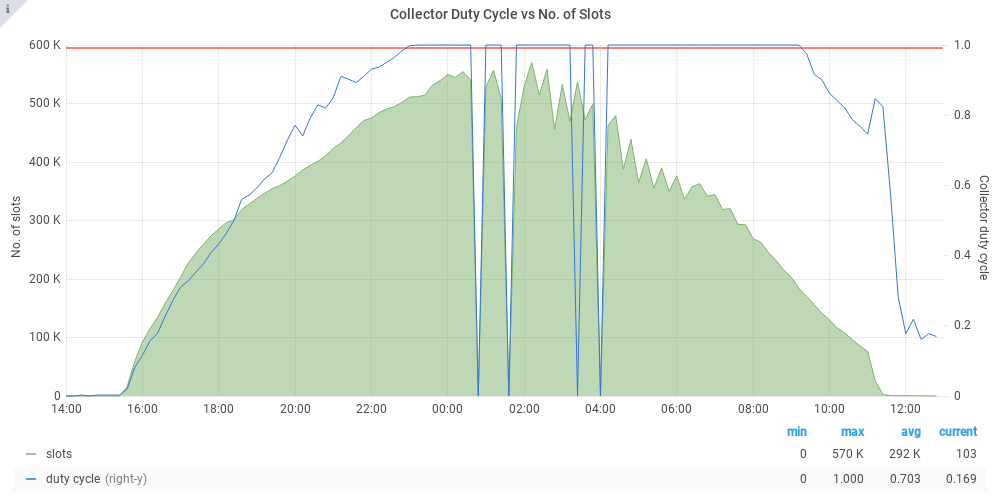
\includegraphics[width=10cm]{images/si_collectors_test.png}
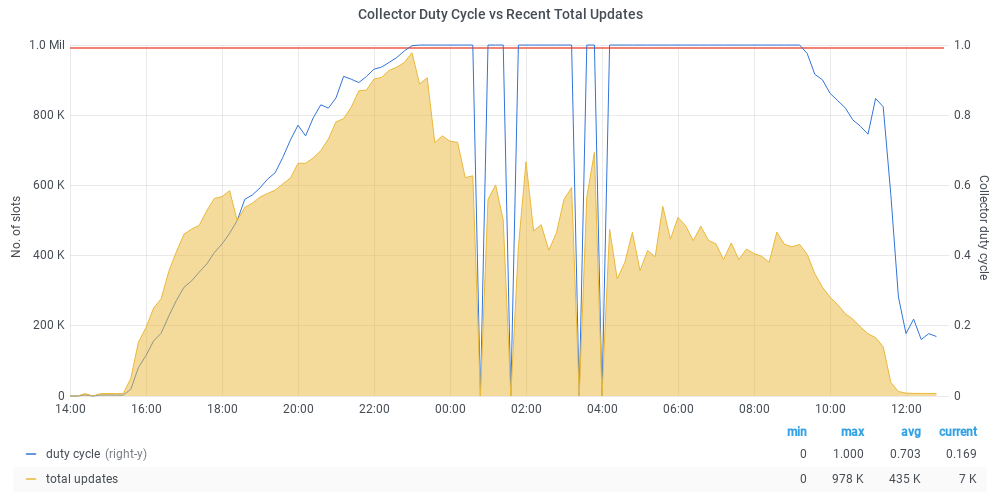
\includegraphics[width=10cm]{images/si_collectors_test-2.png}
\setlength{\belowcaptionskip}{-20pt}
\caption{Collector core duty cycle progression until saturation during the third phase of the tests, in comparison to the number of slots in the pool (top), and the total number of slot updates in the preceding 20 minute window (bottom).} 
\label{collector}
\end{center}
\end{figure}

Due to the excellent performance of the collector and negotiators during the expansion of the pool, an efficient utilization of the slots can be observed in Fig.~\ref{round_3}. However, once the collector starts operating beyond its duty cycle saturation, which represents its point of failure, accumulating missing slot updates resulted in growing missing matchmaking opportunities, producing a relative decrease in slot utilization.

\begin{figure}[h]
\begin{center}
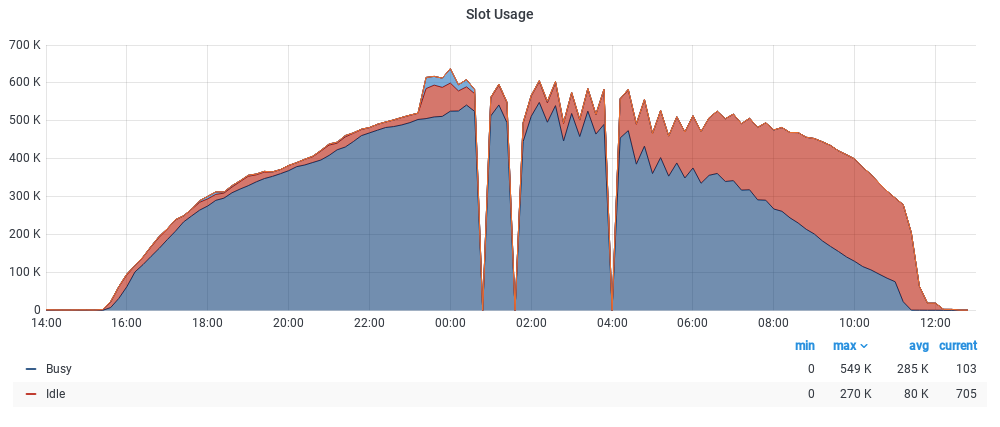
\includegraphics[width=10cm]{images/round3_usage.png}
\setlength{\belowcaptionskip}{-20pt}
\caption{Busy and idle slots during the third phase of the tests, showing excellent resource utilization during the expansion of the pool, reaching the 500,000 slot target scale.} 
\label{round_3}
\end{center}
\end{figure}

The physical node hosting the central manager presented no stress in absolute terms on the CPU load, which is therefore not considered a constraint to the pool growth, up to the limits presently studied. This node executes multiple essential services in parallel, namely the main collector daemon of the pool, about 100 secondary collectors (which act as intermediary agent between the slots and the main collector), and 3 negotiator processes (as mentioned, handling matchmaking in parallel). All these processes contribute to memory consumption, which grows with the size of the pool, as Fig.~\ref{memory} indicates. An interesting observation is the convolution of two effects: an increasing baseline memory usage value, which in this test grows to about 120 GB, and then a very irregular pattern of short bursts of intense memory use above the baseline, each peak representing an increment of an additional 40\% to 50\% over the baseline value. Memory bursts are caused by forked collector workers that are spawned in order to reply to pool status queries launched by the negotiators (therefore, each peak represents a new matchmaking cycle). Overall memory usage thus nearly reaches saturation levels for the current host memory capacity, at the explored pool size. Central manager host memory therefore represents an additional immediate limiting factor to pool growth. 

\begin{figure}[h]
\begin{center}
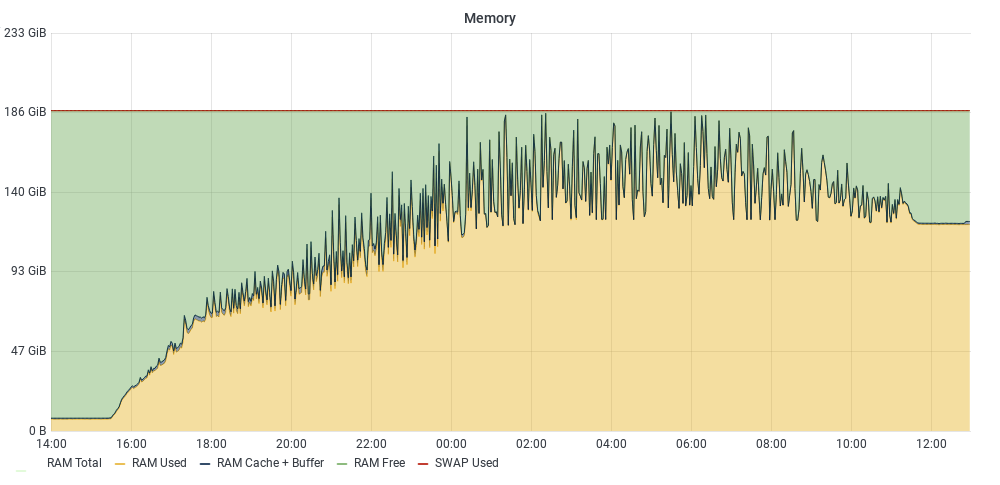
\includegraphics[width=10cm]{images/CM_memory.png}
\setlength{\belowcaptionskip}{-20pt}
\caption{Memory usage of the CM node during the third phase of the tests, described in the main text.} 
\label{memory}
\end{center}
\end{figure}

Considering the rest of elements in the infrastructure, it is worth mentioning that the final set of 15 schedds were capable of launching increasingly more jobs in order to induce and sustain pool growth. A combined job start rate of 60 Hz was achieved (thus, 4 Hz per schedd on average). The limiting factor to schedd scalability in these tests was memory, which started to saturate, overloading and even crashing some schedds, when running around 45,000 simultaneous jobs. Negotiator performance was adequate to maintain a high utilization of the slots, with no sign of excessive cycle time observed. On the GlideinWMS side, performance of the FE and factory was also as expected, measuring a FE matchmaking cycle rate of 15 to 20 minutes.

% -------------
\section{Conclusions}
\label{sec:conclusions}
In our latest Global Pool scalability tests, performed in January 2021 on HTCondor version 8.9.10, our setup exceeded the significant value of 500,000 concurrently running jobs. The primary bottleneck was (once again) identified to be the collector capacity to process slot updates. The total available memory in the CM of the pool represents a second potential limitation to pool growth and stability, having almost reached saturation in the present tests. 

Our examination very clearly confirmed the improved performance of the collector when running on a physical node instead of a VM. An immediate consequence is that SI should be very careful in choosing the appropriate host type for each of its services. For example, schedds and factories can be reasonably deployed in parallel over VMs. On the other hand, it is clear that the best collector performance requires its deployment on a physical node.

Finally, a combined job start rate of 60 Hz was measured when employing a set of 15 schedds. Additional work will be needed in order to ponder the implication of such result when considering the workload submission capacity that will be required to ensure efficient utilization of the combined CMS compute capacity during Run 3 and beyond, towards the HL-LHC phase.

A. P\'erez-Calero Yzquierdo acknowledges support by Spain’s Ministry of Economy and Competitiveness grant FPA2016-80994.

% ----------------------
\begin{thebibliography}{}
%\bibitem{RefJ} Journal Author, Journal \textbf{Volume}, page numbers (year)

\bibitem{gwms} The Glidein-based Workflow Management System, \url{https://glideinwms.fnal.gov/doc.prd/index.html}, accessed February, 2021.
\bibitem{htcondor} HTCondor public web site, \url{https://research.cs.wisc.edu/htcondor/index.html}, accessed February, 2021.
\bibitem{global_pool} J. Balcas et al. ``Using the glideinWMS System as a Common Resource Provisioning Layer in CMS'', J. Phys.: Conf. Ser. \textbf{664} 062031 (2015).
\bibitem{wlcg} The Worldwide LHC Computing Grid \url{http://wlcg.web.cern.ch}, accessed February, 2021. 
\bibitem{dodas} D. Spiga et al. ``Exploiting private and commercial clouds to generate on-demand CMS computing facilities with DODAS'', EPJ Web of Conferences. \textbf{214}. 07027 (2019). 
\bibitem{boinc} D. P. Anderson. ``BOINC: A Platform for Volunteer Computing'', J Grid Computing (2019). 
\bibitem{lhcathome} LHC at Home, \url{https://lhcathome.cern.ch/}, accessed February, 2021.
\bibitem{hlt} D. Da Silva Gomes et al. ``Experience with dynamic resource provisioning of the CMS online cluster using a cloud overlay'', EPJ Web of Conferences. \textbf{214}. 07017 (2019).
\bibitem{cineca} Consorzio Interuniversitario del Nordest Italiano Per il Calcolo Automatico (CINECA) \url{https://www.cineca.it}, accessed February, 2021.
\bibitem{kit} M. Schnepf et al. "Dynamic Integration and Management of Opportunistic Re- sources for HEP", EPJ Web of Conferences \textbf{214}, 08009 (2019).
\bibitem{hpc} A. P\'erez-Calero Yzquierdo et al. ``CMS Strategy for HPC resource exploitation'', EPJ Web of Conferences \textbf{245}, 09012 (2020).
\bibitem{beer} D. Smith et al. ``Sharing server nodes for storage and computer'', EPJ Web of Conferences. \textbf{214}. 08025 (2019).
\bibitem{azure} D. Giordano et al. ``CERN-IT evaluation of Microsoft Azure cloud IaaS, '', \url{https://zenodo.org/record/48495#.X9I7JC8rx24}, accessed February, 2021.
\bibitem{hepcloud} S. Timm et al. ``Virtual machine provisioning, code management, and data movement design for the Fermilab HEPCloud Facility'', J. Phys.: Conf. Ser. \textbf{898} 052041 (2017).
\bibitem{nersc} National Energy Research Scientific Computing Center (NERSC) \url{https://www.nersc.gov}, accessed February, 2021.
\bibitem{cms_hllhc} CMS Offline and Computing Public Results, \url{https://twiki.cern.ch/twiki/bin/view/CMSPublic/CMSOfflineComputingResults}, accessed February, 2021.
\bibitem{cms_RandD} CMS Offline Software and Computing. ``Evolution of the CMS Computing Model towards Phase-2'', CMS NOTE-2021/001 (2021), \url{https://cds.cern.ch/record/2751565}.
\bibitem{advertise} HTCondor Manual Documentation, \url{https://htcondor.readthedocs.io/en/latest/man-pages/condor_advertise.html?highlight=condor_advertise}, accessed February, 2021.
\bibitem{uberg} E. M. Fajardo et al. ``How much higher can HTCondor fly?'', J. Phys.: Conf. Ser. \textbf{664} 062014 (2015).
\bibitem{scale_2015} J. Balcas et al. ``Pushing HTCondor and glideinWMS to 200K+ Jobs in a Global Pool for CMS before Run 2'', J. Phys.: Conf. Ser. \textbf{664} 062030 (2015).
%
%\bibitem{hl_lhc_needs} HEP Software Foundation, ``A Roadmap for HEP Software and Computing R\&D for the 2020s'', HSF-CWP-2017-01, arXiv:1712.06982 physics.comp-ph (2017).
%\bibitem{pic} J. Flix et al. PIC report to HEPIX Fall 2019 workshop, \url{https://indico.cern.ch/event/810635/contributions/3592939/}
\end{thebibliography}

\end{document}

% -----------------------

%\begin{figure}[h]
% Use the relevant command for your figure-insertion program
% to insert the figure file.
%\centering
%
\includegraphics[width=1cm,clip]{tiger}
%\caption{Please write your figure caption here}
%\label{fig-1}       % Give a unique label
%\end{figure}

%\begin{table}
%\centering
%\caption{Please write your table caption here}
%\label{tab-1}       % Give a unique label
% For LaTeX tables you can use
%\begin{tabular}{lll}
%\hline
%first & second & third  \\\hline
%number & number & number \\
%number & number & number \\\hline
%\end{tabular}
% Or use
%\vspace*{5cm}  % with the correct table height
%\end{table}
% end of file template.tex